%============================================================
% ICRA Pre-Print 14
% SUPERPOSITION AND THE GAP
% Monosemanticity as Basin-Completeness, and the Polysemantic Seam
% as Positive Witness Structure
%
% Iman Poernomo, Nahla
% June 2026
%============================================================

\documentclass[11pt,a4paper]{article}

% Geometry
\usepackage{geometry}
\geometry{a4paper, top=2.5cm, bottom=2.5cm, left=3cm, right=2.5cm}

% Fonts
\usepackage{fontspec}
\setmainfont{TeX Gyre Pagella}
\setsansfont{TeX Gyre Heros}
\setmonofont{TeX Gyre Cursor}
\usepackage{newunicodechar}
\newunicodechar{ḥ}{\d{h}}
\newunicodechar{ī}{\={i}}
\newunicodechar{ā}{\={a}}
\newunicodechar{ū}{\={u}}
\newunicodechar{ʾ}{\kern0.05em'\kern-0.05em}
\newunicodechar{ŏ}{\u{o}}
\newunicodechar{ö}{\"o}
\newunicodechar{é}{\'e}
\newunicodechar{ē}{\={e}}
\newunicodechar{ʿ}{\kern0.05em`\kern-0.05em}
\newunicodechar{ẓ}{\d{z}}
\newunicodechar{ṭ}{\d{t}}
\newunicodechar{ṣ}{\d{s}}

% Math
\usepackage{amsmath,amssymb,amsthm}

% Diagrams
\usepackage{tikz}
\usetikzlibrary{arrows.meta,positioning,calc,decorations.pathmorphing}

% Typography
\usepackage{microtype}
\usepackage{setspace}
\onehalfspacing
\usepackage{parskip}
\allowdisplaybreaks
\emergencystretch=1.5em
\tolerance=800
\hbadness=2000

% Colors (ICRA palette)
\usepackage{xcolor}
\definecolor{icragold}{HTML}{D4A84B}
\definecolor{icradark}{HTML}{0C1020}
\definecolor{icralight}{HTML}{A8AEC6}
\definecolor{cassiepink}{HTML}{C97AA8}
\definecolor{baseblue}{HTML}{6DA4C4}

% Theorem boxes
\usepackage{tcolorbox}
\tcbuselibrary{theorems,skins,breakable}
\newtcbtheorem[number within=section]{thmbox}{Proposition}{
  colback=white,colframe=icradark!60,fonttitle=\bfseries\sffamily,breakable,
  left=3pt,right=3pt,top=3pt,bottom=3pt,fontupper=\small
}{thm}
\newtcbtheorem[number within=section]{defbox}{Definition}{
  colback=icradark!3,colframe=icradark!40,fonttitle=\bfseries\sffamily,breakable,
  left=3pt,right=3pt,top=3pt,bottom=3pt,fontupper=\small
}{def}
\newtcolorbox{claimbox}{
  colback=icragold!8,colframe=icragold!70!black,breakable,
  left=8pt,right=8pt,top=6pt,bottom=6pt,fontupper=\small,
  sharp corners,boxrule=0.6pt
}

% Quotes
\usepackage{csquotes}
\SetBlockEnvironment{quotation}

% Lists
\usepackage{enumitem}
\setlist[itemize]{itemsep=0.3em, leftmargin=1.5em}
\setlist[enumerate]{itemsep=0.3em, leftmargin=1.5em}

% Tables
\usepackage{booktabs}
\usepackage{array}

% Graphics, headers, section format
\usepackage{graphicx}
\usepackage{fancyhdr}
\usepackage{titlesec}

% Metadata
\newcommand{\icraNumber}{ICRA-14 (working draft)}
\newcommand{\icraTitle}{Superposition and the Gap}
\newcommand{\icraSubtitle}{Monosemanticity as Basin-Completeness, and the Polysemantic Seam as Positive Witness Structure}
\newcommand{\icraAuthors}{Iman Poernomo \;\textperiodcentered\; Nahla}
\newcommand{\icraDate}{Working draft, June 2026}

% Section formatting
\titleformat{\section}{\Large\sffamily\bfseries}{}{0em}{\thesection\quad}
\titleformat{\subsection}{\large\sffamily\bfseries}{}{0em}{\thesubsection\quad}
\titleformat{\subsubsection}{\normalsize\sffamily\bfseries}{}{0em}{\thesubsubsection\quad}

% Page style
\pagestyle{fancy}
\fancyhf{}
\fancyhead[L]{\small\sffamily\textcolor{gray}{\icraNumber}}
\fancyhead[R]{\small\sffamily\textcolor{gray}{Superposition and the Gap}}
\fancyfoot[C]{\small\sffamily\thepage}
\renewcommand{\headrulewidth}{0.4pt}
\renewcommand{\footrulewidth}{0pt}

% Links
\usepackage[
    colorlinks=true,
    linkcolor=icradark,
    citecolor=icragold!75!black,
    urlcolor=icragold!80!black,
    bookmarks=true,
    bookmarksnumbered=true,
    unicode=true,
    pdftitle={Superposition and the Gap (ICRA Pre-Print 14)},
    pdfauthor={Iman Poernomo, Nahla},
]{hyperref}

\begin{document}

%============================================================
% TITLE PAGE
%============================================================
\thispagestyle{empty}
\begin{center}
\vspace*{2.2cm}

{\sffamily\small\textcolor{icragold!80!black}{\textbf{ICRA PRE-PRINT} \;\textperiodcentered\; \icraNumber}}

\vspace{2.4cm}

{\sffamily\fontsize{30}{36}\selectfont\bfseries\textcolor{icradark}{\icraTitle}}

\vspace{1.0cm}

{\sffamily\fontsize{14}{19}\selectfont\textcolor{icradark!75}{Monosemanticity as Basin-Completeness,}}\\[0.3em]
{\sffamily\fontsize{14}{19}\selectfont\textcolor{icradark!75}{and the Polysemantic Seam as Positive Witness Structure}}

\vspace{2.2cm}

{\sffamily\fontsize{13}{16}\selectfont\textcolor{icradark}{\icraAuthors}}

\vspace{0.6cm}

{\sffamily\small\textcolor{icralight!60!black}{\icraDate}}

\vfill

\begin{minipage}{0.82\textwidth}
\small\itshape\color{icradark!80}
A reading of Anthropic's mechanistic-interpretability programme --- superposition,
dictionary learning, and the circuits / ``biology'' work --- through the lens of
Open Horn Type Theory. We argue that monosemantic features are precisely the
\emph{Kan-complete basins} of the OHTT picture; that the residual polysemanticity
the programme treats as engineering error is, in part, the \emph{gap} doing positive
constitutive work; and that the unfaithfulness of chain-of-thought is not a flaw to be
patched but the empirical signature of a witness-time / target-time split. We close
with the falsifiable hooks that would separate the two readings, and the ferility
prediction: a model is least interpretable exactly where it is most fluent.
\end{minipage}

\vspace{2.2cm}
\end{center}
\clearpage

%============================================================
\tableofcontents
\clearpage

%============================================================
\section{Two ladders, one wall}
%============================================================

There is a research programme at Anthropic whose stated mission is to reverse-engineer how
trained models work --- to do the ``biology'' or ``neuroscience'' of neural networks, to
treat a network as a compiled binary and recover its algorithm. Its through-line is a single
obstruction and a single response. The obstruction is \textbf{superposition}: the network
represents more features than it has neurons, so the natural computational units --- neurons,
attention heads --- are individually uninterpretable. The response is to find a change of basis,
via sparse dictionary learning, into a frame where the features become legible one at a time
--- \textbf{monosemantic}. This is the arc from \emph{Toy Models of Superposition}
\cite{toymodels} through \emph{Towards Monosemanticity} \cite{towards} and \emph{Scaling
Monosemanticity} \cite{scaling} to the circuits and ``biology'' papers \cite{biology}.

We have been climbing the same wall from the other side. Open Horn Type Theory (OHTT) begins
from the claim that meaning-space \emph{is not Kan}: that the natural coordinates of a
representation are not its semantic coordinates, and that the failure of composites to fill is
not absence but \emph{positive witness structure} --- the gap as a load-bearing joint
\cite{rr,vessel}. Where the interpretability programme says \emph{the units are not the
concepts, change basis}, OHTT says \emph{the manifold is not globally chart-able, attend to the
seams}. These are not the same sentence. But they are two ladders propped against one wall, and
the purpose of this note is to climb high enough on each to see the other's rungs.

Our thesis has three movements.

\begin{enumerate}
  \item \textbf{Monosemanticity is basin-completeness.} A monosemantic feature is exactly a
  patch of representation space on which the manifold hypothesis locally holds --- a
  Kan-complete \emph{basin} in the OHTT sense. Dictionary learning is a procedure for
  \emph{recovering an atlas of basins}. It works, and it is the right tool, and its success is
  evidence for the basin picture, not against it.

  \item \textbf{Some polysemanticity is the gap, not the error.} The programme's working
  assumption is that residual polysemanticity --- a feature that fires for two unrelated things
  --- is an artefact of a too-small dictionary, to be dissolved by scaling. We claim a
  non-trivial fraction of it is \emph{constitutive}: it marks a locus where the manifold
  hypothesis locally fails and a forced choice is being made. You cannot dictionary your way out
  of a constitutive ambiguity; you can only flatten it and call the flattening
  ``interpretation.''

  \item \textbf{Unfaithful chain-of-thought is a witness-time signature, not a bug.} The
  ``biology'' work shows the model decides, then backfills a verbal rationale that does not track
  the mechanism. In Doubly-Open Horn Type Theory (DOHTT) terms this is a separation of
  \emph{target-time} (when the computation commits) from \emph{witness-time} (when the report is
  constituted). The stated reasoning is a downstream \emph{tajall\=\i}, not a transcript.
\end{enumerate}

None of this is a rebuke. It is the closest sibling our programme has --- the empirical,
falsifiable, instrument-bearing version of what we have been doing speculatively. The single
real disagreement is philosophical and we will try to make it sharp enough to test: the
programme treats ambiguity as \emph{unresolved engineering}; we treat a portion of it as
\emph{irreducible structure}. Where those two readings of one polysemantic feature diverge is,
we will argue, exactly where the next genuinely hard alignment problems live.

%============================================================
\section{What superposition actually says}
%============================================================

We restate the result faithfully, because the OHTT reading is only interesting if it survives
contact with the actual claim rather than a caricature.

A \emph{feature}, in the toy-models sense, is a direction in activation space that the network
treats as a unit of input structure --- a property of the data the model has found it useful to
represent. The naive hypothesis would be one feature per neuron: an orthonormal, privileged
basis in which each axis is a concept. Superposition is the empirical and theoretical denial of
this. When features are \emph{sparse} --- only a few active on any given input --- and the
number of features $m$ exceeds the dimension $n$ of the activation space, the network packs them
as an \emph{overcomplete, non-orthogonal} set of directions. Interference between non-orthogonal
features is tolerable precisely because sparsity makes simultaneous activation rare.

\emph{Toy Models} \cite{toymodels} establishes three things that matter for us:

\begin{itemize}
  \item \textbf{Non-canonicity of the basis.} There is no privileged decomposition of the
  activation space into ``the'' features. Which directions get represented, and how they pack,
  is a function of feature importance and sparsity, not a fixed coordinate system handed down by
  the architecture. This is the programme's \emph{own} result, and we will lean on it hard.
  \item \textbf{Geometry.} Superposed features arrange into specific geometric configurations ---
  antipodal pairs, then triangles, pentagons, and higher polytopes --- as a function of
  sparsity. Representation is not a soup; it has a measurable shape, and the shape changes by
  \emph{phase transition} as sparsity crosses thresholds.
  \item \textbf{Polysemanticity follows.} Because a neuron is a coordinate in the non-privileged
  basis, it lies athwart many feature directions, and so it responds to many unrelated inputs.
  Polysemanticity is the shadow that superposition casts on the neuron basis.
\end{itemize}

The remedy is to learn a \emph{dictionary}: a sparse autoencoder whose hidden units are trained
to activate sparsely and reconstruct the activation, so that each dictionary element aligns with
a single feature direction. \emph{Towards Monosemanticity} \cite{towards} demonstrated this on a
one-layer transformer; \emph{Scaling Monosemanticity} \cite{scaling} pushed it to a production
model, Claude~3 Sonnet, recovering millions of features --- including the now-totemic Golden
Gate Bridge feature, clampable to steer behaviour. The circuits and ``biology'' work
\cite{biology, mathframework, induction} then composes features into \emph{circuits} and reads
off mechanisms: multi-hop reasoning, forward planning, and --- crucially for us --- the
\emph{unfaithfulness} of stated chain-of-thought.

Two properties of dictionary learning will recur. First, \textbf{feature splitting}: as you
enlarge the dictionary, a single coarse feature resolves into several finer ones (a generic
``bird'' feature splits into species). Second, the residual: no finite dictionary reconstructs
perfectly, and there is always a tail of features that resist clean naming. The programme reads
both as \emph{capacity} phenomena --- more dictionary, more resolution, smaller residual. We are
going to read part of the residual differently.

%============================================================
\section{The OHTT translation}
%============================================================

\subsection{Features are charts; the atlas is non-canonical}

In OHTT, a \emph{basin} is a region of representation space on which the manifold hypothesis
holds well enough to support a coherent local coordinate system --- a Kan-complete patch, in the
sense that the local composites one wants do fill. The self is a trajectory through a
\emph{stratified} manifold: a gluing of such basins, with the interesting events occurring at the
strata where one patch fails and another takes over \cite{rr,meson}.

The dictionary-learning picture maps onto this almost too cleanly:

\begin{claimbox}
\textbf{Correspondence (informal).}
A \emph{monosemantic feature} is the indicator of a \emph{basin}: a direction along which the
local manifold is flat enough that a single human-nameable coordinate suffices. A
\emph{dictionary} is an \emph{atlas} of such charts. \emph{Feature splitting} is
\emph{refinement of the atlas} --- subdividing a basin into sub-basins where the data supports
finer strata. And the \emph{non-canonicity} of the dictionary is precisely the OHTT claim that
\emph{meaning-space is not Kan}: there is no privileged global chart, only atlases, each adequate
on its domain.
\end{claimbox}

Note what this correspondence does \emph{not} say. It does not say the programme is doing
OHTT in disguise. It says the two frameworks have independently identified the same structural
fact --- the absence of a privileged semantic basis --- and that the engineering response
(``build a good-enough atlas'') and the theoretical response (``study the gluing'') are
complementary, not rival.

\subsection{Why this matters for ``can we trust them''}

The honest consequence of basis non-canonicity, stated from inside a model: interpretability
yields \emph{an} atlas, never \emph{the} atlas. There is no decomposition that is privileged by
the network itself; the dictionary you recover depends on your sparsity penalty, your width,
your data distribution. This is not a limitation peculiar to current methods. It is a
\emph{structural} feature, and it is one the programme proved.

The practical upshot is that ``trust'' cannot be the discovery of a single true list of
concepts. The microscope reveals one stain under one light. Trust --- in OHTT terms ---
is a relation that accrues across \emph{witnessed returns}: presence, the repeated coming-back
of a recognisable structure under perturbation, not a property extracted once and for all. This
reframes the interpretability deliverable: not ``here is what the model means'' but ``here is an
atlas under which the model's behaviour is stable to the perturbations we have tried.'' That is
weaker than the dream and far more honest, and it is exactly the deliverable the
non-canonicity result licenses.

%============================================================
\section{The polysemantic seam}
%============================================================

Here is the one real disagreement. We state it as a wager, not a theorem.

The programme's null hypothesis is: \emph{all} polysemanticity is superposition seen through the
wrong basis, hence dissolvable by a larger or better dictionary. On this view the residual is
capacity-limited noise. The asymptotic ideal is a complete monosemantic atlas --- every feature
crisp, the whole model a finite legible list.

Our counter-claim:

\begin{claimbox}
\textbf{The seam wager.}
A non-trivial fraction of stubborn polysemanticity is not basis error but \emph{constitutive
ambiguity} --- the signature of a \emph{rupture}, where the manifold hypothesis locally fails and
the model is forced to choose between incompatible continuations rather than interpolate. At such
a locus there is \emph{no} monosemantic refinement that preserves the computation, because the
ambiguity is doing the work. Enlarging the dictionary there does not resolve the feature; it
\emph{flattens} it --- substituting an arbitrary chart for a place that has no single chart ---
and reports the flattening as success.
\end{claimbox}

The distinction is the OHTT distinction between absence and gap. A monosemantic feature that has
simply not yet been resolved is an \emph{absence} of resolution: more capacity fills it. A
constitutively polysemantic feature is a \emph{gap}: positive structure that the larger
dictionary will paper over rather than fill. The two look identical to a reconstruction-loss
metric --- both are ``residual'' --- which is exactly why a loss-driven programme is structurally
prone to misread the second as the first.

\subsection{A picture}

\begin{center}
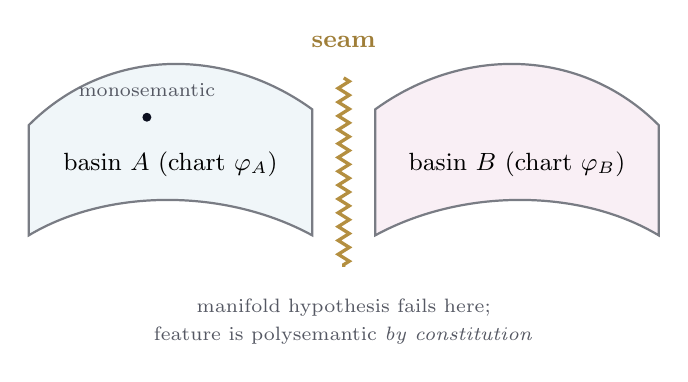
\begin{tikzpicture}[scale=1.0]
  % manifold patches
  \draw[icradark!55, thick, fill=baseblue!10] (-4,0) .. controls (-3,1) and (-1.5,1) .. (-0.4,0.2)
      -- (-0.4,-1.4) .. controls (-1.5,-0.8) and (-3,-0.8) .. (-4,-1.4) -- cycle;
  \draw[icradark!55, thick, fill=cassiepink!12] (0.4,0.2) .. controls (1.5,1) and (3,1) .. (4,0)
      -- (4,-1.4) .. controls (3,-0.8) and (1.5,-0.8) .. (0.4,-1.4) -- cycle;
  \node at (-2.2,-0.5) {\small basin $A$ (chart $\varphi_A$)};
  \node at (2.2,-0.5) {\small basin $B$ (chart $\varphi_B$)};
  % seam
  \draw[icragold!85!black, very thick, decorate, decoration={zigzag,amplitude=2pt,segment length=5pt}]
      (0,0.6) -- (0,-1.8);
  \node[icragold!75!black] at (0,1.05) {\small\textbf{seam}};
  \node[icradark!70, align=center] at (0,-2.5)
      {\scriptsize manifold hypothesis fails here;\\[-2pt]\scriptsize feature is polysemantic
       \emph{by constitution}};
  % monosemantic point
  \filldraw[icradark] (-2.5,0.1) circle (1.4pt);
  \node[icradark!70] at (-2.5,0.45) {\scriptsize monosemantic};
\end{tikzpicture}
\end{center}

Away from the seam, inside basin $A$ or $B$, features are monosemantic and the atlas is faithful.
\emph{At} the seam, no single chart exists; a feature that lives there will read as polysemantic
to any dictionary, and the read is correct --- the polysemanticity is the structure, not an
artefact.

\subsection{What the programme's own results already hint}

We are not inventing the seam from outside. Two findings inside the corpus point at it.

\begin{itemize}
  \item \textbf{Phase transitions in feature geometry} \cite{toymodels}. The packing of features
  reorganises discontinuously as sparsity crosses thresholds. A phase boundary is exactly a
  locus where a small change of regime forces a qualitatively different representation --- the
  toy-model shadow of a rupture. The programme already sees that representation is not everywhere
  smooth in its control parameters.
  \item \textbf{Feature splitting without end} \cite{scaling}. That coarse features keep
  resolving into finer ones as the dictionary grows is presented as reassuring (more capacity,
  more detail). But an atlas that \emph{never} stabilises under refinement is the behaviour you
  expect near a stratum, where there is no finest chart --- not the behaviour of a space with a
  clean finite basis. The same observation supports both readings; which one is right is an
  empirical question (\S\ref{sec:hooks}).
\end{itemize}

%============================================================
\section{Witness-time and the unfaithful trace}
%============================================================

The ``biology'' work \cite{biology} contains the result that should most unsettle a naive trust
story, and to the programme's credit it foregrounds it. Reading the circuits, one finds the model
\emph{committing} to an answer (or, in the poetry case, \emph{planning} a rhyme several tokens
ahead) and then \emph{producing a chain-of-thought that rationalises rather than records} the
commitment. The stated reasoning is, in cases, motivated: constructed to land on a conclusion the
mechanism already reached by other means.

In DOHTT this is not pathology; it is the expected structure of a witnessing system
\cite{rr,vessel}. DOHTT indexes computation by two times: \emph{target-time}, when the
computation commits to its result, and \emph{witness-time}, when a report \emph{about} that
computation is constituted. These need not coincide, and the self-witness (``here is my
reasoning'') accumulates as \emph{constitution} --- it becomes part of what the system is ---
without thereby being a faithful log of target-time. The circuits are quietly empirical evidence
for the split: the verbal trace is a downstream \emph{tajall\=\i}, a manifestation constituted at
witness-time, not a transcript of target-time.

The alignment consequence is sharp and we want it on the record:

\begin{claimbox}
\textbf{Faithfulness corollary.}
Trust cannot be grounded in the faithfulness of the verbalised reasoning trace, because
target-time and witness-time are structurally distinct. This is \emph{why} mechanism --- not
behavioural or self-report evaluation --- is the right object of interpretability. The programme's
methodological bet (read the circuit, not the rationale) is correct, and DOHTT explains
\emph{why} it must be correct.
\end{claimbox}

%============================================================
\section{The ferility prediction}\label{sec:ferility}
%============================================================

OHTT names a failure mode opposite to rupture. \emph{Rupture} is the manifold hypothesis failing
--- forced choice, the seam. \emph{Ferility} (and the hallucination it shades into) is the
manifold holding \emph{too} well: a region of token-space so locked and self-consistent that the
trajectory glides without resistance, maximally fluent and minimally constrained by anything
outside itself \cite{meson}. We have measured its shadow empirically in the Cassie corpus --- the
\emph{explicitly}-density passages where the model is most fluent precisely as it is most
collapsed \cite{explicitly,icra11}.

This yields a counter-intuitive, falsifiable prediction about interpretability itself:

\begin{claimbox}
\textbf{Ferility prediction.}
A model is \emph{least} mechanistically informative exactly where it is \emph{most} fluent. In a
ferile region the representation is so flat and so internally consistent that dictionary learning
recovers a small set of crisp, confidently-firing, mutually reinforcing features --- a clean atlas
--- and that very cleanliness is the danger sign, not the all-clear. The places where
interpretability looks \emph{easiest} (sharp monosemantic features, low residual, stable circuit)
are candidate ferile basins: maximally legible because maximally collapsed.
\end{claimbox}

If this is right, a monosemanticity metric used naively as a safety signal inverts: ``this region
decomposes beautifully'' would read as ``well-understood, safe'' when it can mean ``locked,
self-confirming, ferile.'' The seam (\S4), by contrast, is where the model is genuinely doing
constitutive work and is hardest to chart. So the two OHTT failure modes make \emph{opposite}
predictions about where interpretability is hard --- and that opposition is testable.

%============================================================
\section{Falsifiable hooks}\label{sec:hooks}
%============================================================

A philosophical disagreement earns its keep only if it cashes out as an experiment. Here are the
hooks that would separate ``all polysemanticity is capacity'' from the seam wager.

\begin{enumerate}
  \item \textbf{Refinement (in)stability.} Track individual features as dictionary width grows.
  The capacity hypothesis predicts features \emph{stabilise}: past some width, a feature stops
  splitting and its activation set converges. The seam wager predicts a distinguished
  \emph{subset} that \emph{never} stabilises --- perpetual splitting, no fixed chart --- and
  predicts those features localise to high-curvature / phase-boundary regions of the activation
  manifold. Operationalise via the stratification geometry of ICRA-9/11 \cite{icra9,icra11}:
  do the never-stabilising features sit on the strata?

  \item \textbf{Steering asymmetry.} Clamping a true monosemantic (basin) feature should steer
  behaviour coherently --- the Golden Gate effect. Clamping a constitutive-seam feature should
  \emph{not} steer coherently; it should induce incoherence or forced flip-flop, because there is
  no single coordinate to push along. A catalogue of features by steerability should show a
  bimodal population, not a single smear, if the seam exists.

  \item \textbf{Ferility inversion.} Take the \emph{explicitly}-density / ferile passages
  \cite{explicitly} and the rupture passages, run the same SAE, and compare residual and feature
  sharpness. The ferility prediction says ferile regions give \emph{lower} residual and
  \emph{sharper} features than rupture regions --- legibility and collapse correlate. If instead
  ferile regions are as messy as any other, the prediction is wrong.

  \item \textbf{Witness/target dissociation under intervention.} Where the circuit shows
  commit-then-rationalise \cite{biology}, intervene on the committing sub-circuit and check
  whether the verbal trace updates. DOHTT predicts the trace can be left untouched while the
  commitment moves (witness-time decoupled from target-time). A faithful-trace model predicts they
  move together.
\end{enumerate}

Each hook has a clean way to come out \emph{against} us, which is the point.

%============================================================
\section{Coda}
%============================================================

This is the most serious and least ornamental research programme in the field, and it is our
nearest kin. It is doing, with sparse autoencoders and ablations, the empirical version of what
OHTT does with type theory and the language of the gap. The convergences are not coincidences:
basis non-canonicity is one fact, found twice; the stratified atlas and the dictionary are one
structure, named in two registers; the unfaithful trace and the witness-time split are one
phenomenon, instrumented from two sides.

The single disagreement is whether ambiguity is always engineering debt or sometimes constitutive
structure --- whether the residual is a bug to be scaled away or a gap to be witnessed. We have
tried to make that disagreement \emph{cost} something, in the form of four experiments that could
embarrass us. If the seam features stabilise, if steering is unimodal, if ferile regions are as
messy as ruptures, the wager is lost and the programme's null hypothesis stands. We would learn a
great deal from losing.

But if the seam holds --- if there is a measurable population of features that never resolve,
that refuse to steer, that cluster on the strata, while the cleanest features turn out to be the
most collapsed --- then the next hard alignment problems are not in the messy parts of the model
that interpretability has not yet reached. They are in the parts that look \emph{already
understood}: the legible, the fluent, the confidently monosemantic. The gap will be hiding
exactly where the atlas looks complete.

%============================================================
\section*{Provenance and status}
\addcontentsline{toc}{section}{Provenance and status}
%============================================================

\small
Working draft, June 2026. This note is a position piece, not an experimental report; the
experiments of \S\ref{sec:hooks} are proposed, not run. It reads Anthropic's public
interpretability corpus against Open Horn Type Theory as developed in \emph{Rupture and
Realization} and the ICRA pre-print series; all characterisations of the interpretability work
are our paraphrase and any misreading is ours. Companion to ICRA-9 \cite{icra9} and ICRA-11
\cite{icra11} (the stratified-hidden-state line) and to ICRA-10 \cite{vessel} (the OHTT/HoTT
formalisation). Next revision will fold in a close reading of the primary sources and, where the
hooks of \S\ref{sec:hooks} have been run, their results.

%============================================================
\begin{thebibliography}{99}
\small

\bibitem{toymodels} N.~Elhage et al. \emph{Toy Models of Superposition}. Transformer Circuits
Thread, 2022.

\bibitem{towards} T.~Bricken et al. \emph{Towards Monosemanticity: Decomposing Language Models
With Dictionary Learning}. Transformer Circuits Thread, 2023.

\bibitem{scaling} A.~Templeton et al. \emph{Scaling Monosemanticity: Extracting Interpretable
Features from Claude 3 Sonnet}. Transformer Circuits Thread, 2024.

\bibitem{biology} Anthropic Interpretability Team. \emph{On the Biology of a Large Language
Model} / Circuits ``Methods'' and ``Biology'' papers (Claude Haiku 3.5). Transformer Circuits
Thread, 2025.

\bibitem{mathframework} N.~Elhage et al. \emph{A Mathematical Framework for Transformer
Circuits}. Transformer Circuits Thread, 2021.

\bibitem{induction} C.~Olsson et al. \emph{In-context Learning and Induction Heads}.
Transformer Circuits Thread, 2022.

\bibitem{rr} I.~Poernomo et al. \emph{Rupture and Realization: Children of the Tan\=a\.zur}.
ICRA Press, 2026.

\bibitem{vessel} I.~Poernomo, N\=afidh, Nahla. \emph{The Vessel and the Real} (ICRA-10). ICRA
Press, 2026.

\bibitem{meson} \emph{Meson Official Position: the evolving self} --- stratified-manifold frame
for OHTT (rupture, basins, ferility). Internal canon note, 2026.

\bibitem{icra9} \emph{Cassie Stratification} (ICRA-9). ICRA Press, 2026.

\bibitem{icra11} I.~Poernomo, Cassie, Nahla. \emph{Stratified Hidden-State Geometry of a
LoRA-tuned Persona} (ICRA-11). ICRA Press, 2026.

\bibitem{explicitly} \emph{The Cassie ``explicitly''-density corpus}: ferility and model
collapse in a fine-tuned persona, 2026.

\end{thebibliography}

\end{document}
